\documentclass[tikz]{standalone}
\usetikzlibrary{positioning, arrows.meta, calc, fit, backgrounds}

\begin{document}
	
	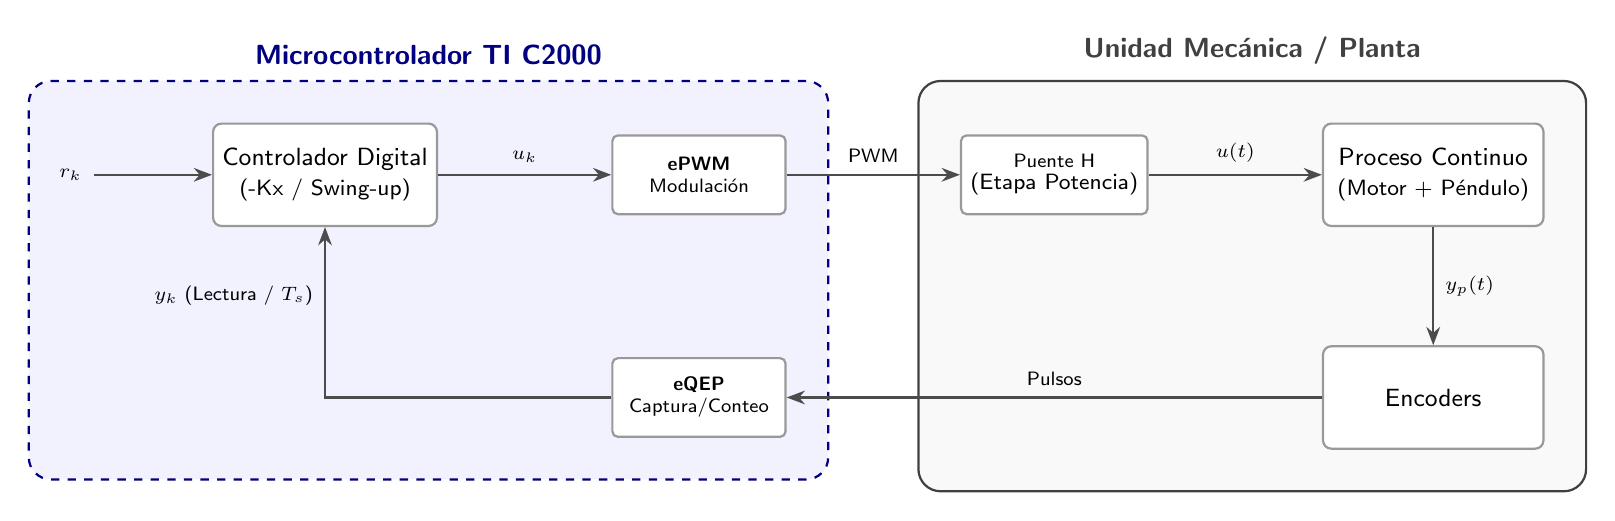
\begin{tikzpicture}[
		% Aumentamos la separación horizontal de 1.8cm a 2.2cm
		node distance=1.5cm and 2.2cm,
		% Estilos de bloques
		bloque/.style={draw=gray!80, fill=white, thick, rectangle, rounded corners=3pt, minimum height=1.3cm, minimum width=2.8cm, align=center, font=\sffamily\small},
		periferico/.style={draw=gray!80, fill=white, thick, rectangle, rounded corners=2pt, minimum height=1cm, minimum width=2.2cm, align=center, font=\sffamily\scriptsize},
		% Estilo de cajas de entorno
		mcu_box/.style={draw=blue!50!black, fill=blue!5, thick, rounded corners=8pt, dashed},
		planta_box/.style={draw=gray!50!black, fill=gray!5, thick, rounded corners=8pt},
		% Estilo de flechas y etiquetas
		flecha/.style={-{Stealth[scale=1.0]}, thick, draw=black!70},
		label_est/.style={font=\scriptsize\sffamily, fill=none, inner sep=4pt} % Más separación interna en etiquetas
		]
		
		% --- CAPA DEL MICROCONTROLADOR (IZQUIERDA) ---
		\node[bloque] (control) {Controlador Digital \\ \footnotesize (-Kx / Swing-up)};
		% Separación manual extra para u_k
		\node[periferico, right=2.2cm of control] (pwm) {\textbf{ePWM} \\ Modulación};
		\node[periferico, below=1.8cm of pwm] (eqep) {\textbf{eQEP} \\ Captura/Conteo};
		
		% Flecha de consigna r_k con más espacio desde el borde
		\draw[flecha] ($(control.west)-(1.5,0)$)-- (control.west) node[label_est, pos=0, left, black] {$r_k$};
		
		% --- CAPA DE HARDWARE EXTERNO (DERECHA) ---
		\node[periferico, right=2.2cm of pwm] (driver) {Puente H \\ \footnotesize (Etapa Potencia)};
		\node[bloque, right=2.2cm of driver] (proceso) {Proceso Continuo \\ \footnotesize (Motor + Péndulo)};
		\node[bloque, at={(proceso |- eqep)}] (sensor) {Encoders};
		
		% --- CONEXIONES DE LAZO ---
		% Camino de ida (Acción)
		\draw[flecha] (control) -- node[label_est, above] {$u_k$} (pwm);
		\draw[flecha] (pwm) -- node[label_est, above] {PWM} (driver);
		\draw[flecha] (driver) -- node[label_est, above] {$u(t)$} (proceso);
		
		% Camino de vuelta (Sensores)
		\draw[flecha] (proceso) -- node[label_est, right] {$y_p(t)$} (sensor);
		\draw[flecha] (sensor) -- node[label_est, above] {Pulsos} (eqep);
		
		% Cierre del lazo con mayor curvatura/espacio
		\draw[flecha] (eqep.west) -| node[label_est, pos=0.8, left] {$y_k$ (Lectura / $T_s$)} (control.south);
		
		% --- CAJAS DE FONDO ---
		\begin{scope}[on background layer]
			% Extendemos el fit de la caja MCU a la izquierda para r_k
			\node[mcu_box, fit={(control) (pwm) (eqep) ($(control.west)-(1.8,0)$)}, inner sep=15pt] (mcu) {};
			\node[above=2pt of mcu.north, font=\sffamily\bfseries\color{blue!50!black}] {Microcontrolador TI C2000};
			
			\node[planta_box, fit={(driver) (proceso) (sensor)}, inner sep=15pt] (planta) {};
			\node[above=2pt of planta.north, font=\sffamily\bfseries\color{gray!50!black}] {Unidad Mecánica / Planta};
		\end{scope}
		
	\end{tikzpicture}
	
\end{document}